%!TEX TS-program = xelatex
%!TEX root = ../../maxwell2018thesis.tex

\begin{tikzpicture}[remember picture, overlay]
      \node[anchor=north west] at (-2.88,3.475){%
        \scalebox{0.66}{\pgfimage{figures/ch0-acks_header.pdf}}};
\end{tikzpicture}

\begin{preamble}[The PhD Journey]
\phantomsection
\addcontentsline{toc}{part}{The PhD Journey}

% \resizebox{1\hsize}{!}{
% 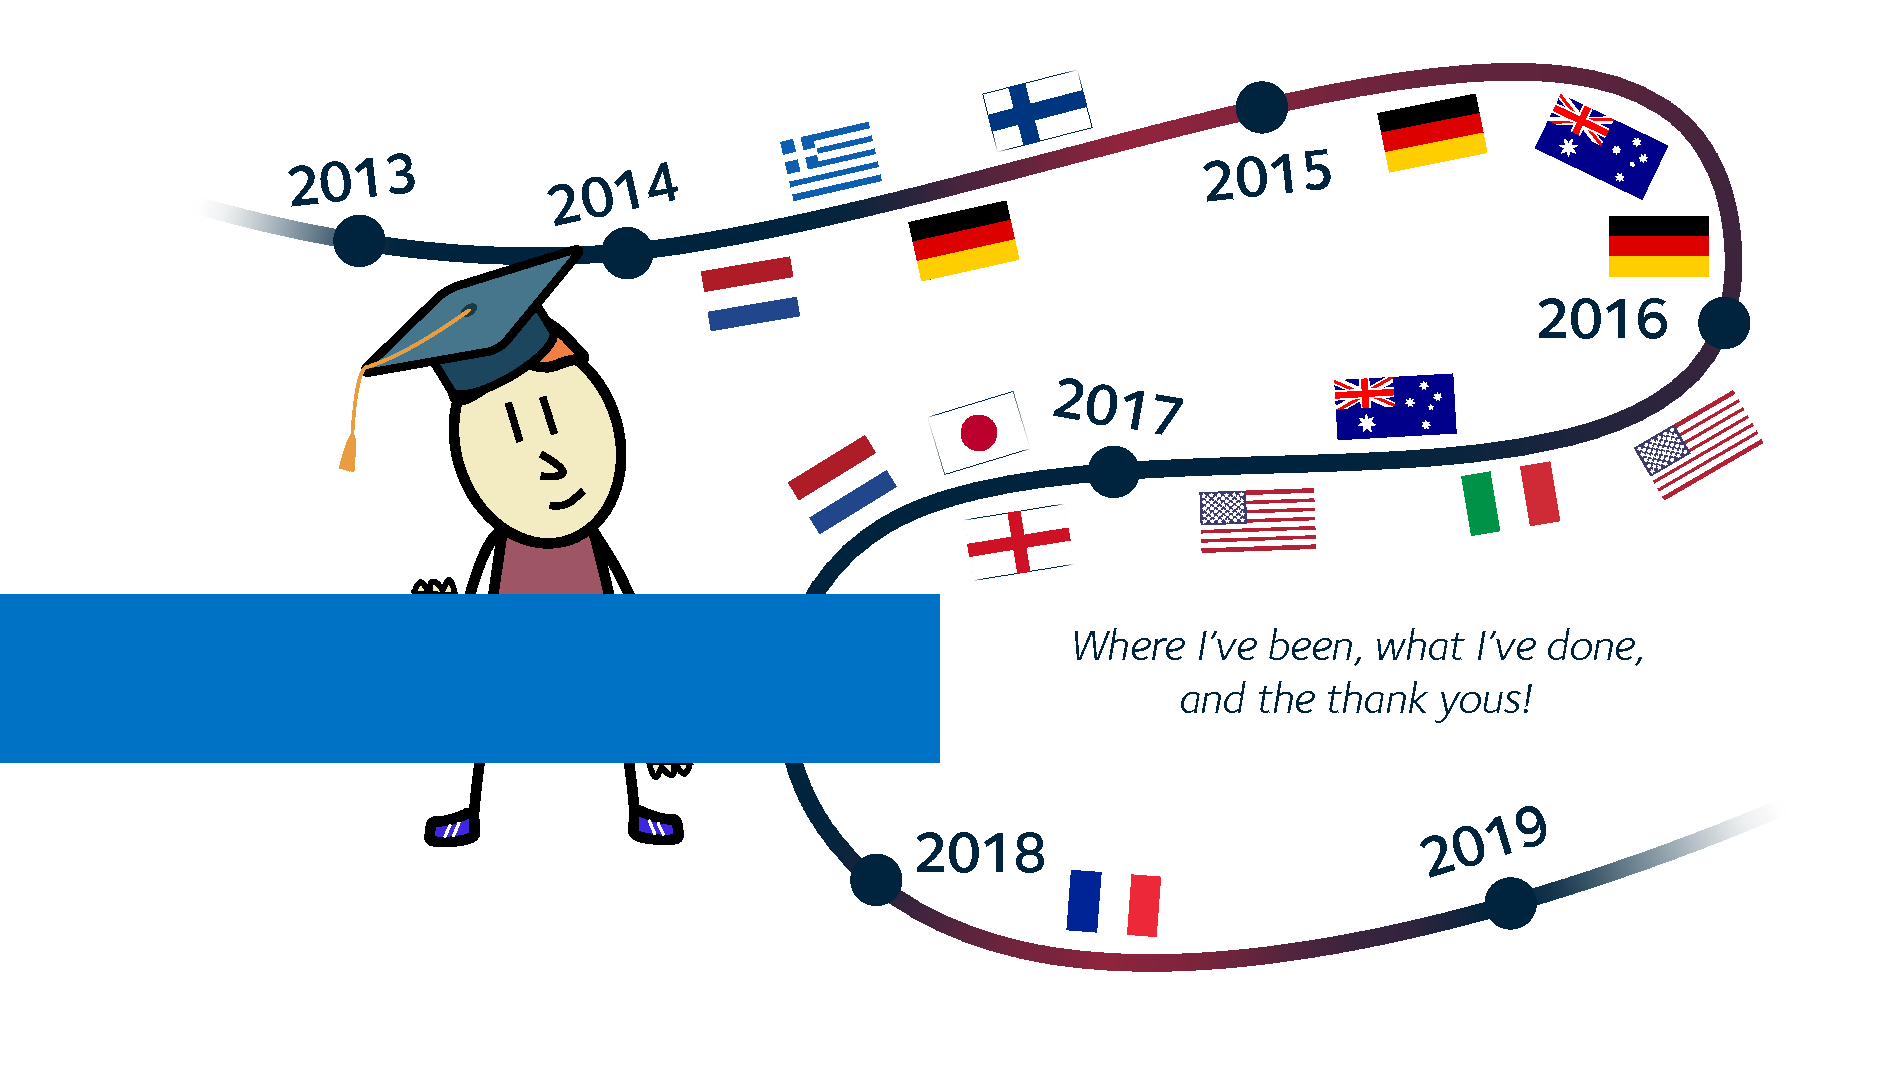
\includegraphics{figures/ch0-acks_header.pdf}}

A good friend of mine -- and a fellow PhD student -- once said to me that when the time came to write his PhD thesis, he would avoid an acknowledgements section where \emph{everyone and their dog} would be thanked for helping him reach his ultimate goal of attaining a PhD. I on the other hand take a very different light on this matter. There are a lot of people who have in one way or another helped me reach where I am today. Whether these people actively guided me in my studies, or were individuals who I was fortunate to meet and simply have a drink with throughout the past five years, they all \emph{``cajoled''}\footnote{I like this term. Professor Ian Ruthven used it in his PhD thesis~\citep{ruthven2001phd} as a means of describing the individuals who were there for him, behind the scenes, ``cajoling'' him to complete his thesis.} me in one way or another towards the finishing line.

I firmly believe that everybody who I have had the pleasure of meeting and working with over the past five years should be acknowledged -- whether or not they feel they contributed in any meaningful way. If you are one of these people and are left wondering, believe me: \emph{you did make a difference.} \textbf{\emph{To show my sincere appreciation, I want to dedicate this work to each and every one of them}} -- regardless of whether they have a dog or not.

Hindsight tells me that doing a PhD is much like embarking on a \emph{very long,} solo journey. Unless you do one yourself, you won't appreciate how tough (and lonely) it can be at times. Three years in, you might find yourself sitting in your lab by yourself on a Friday night, wondering why your experiments aren't producing the results you expect. It can all seem so very pointless, and you question why you're doing what you're doing. I experienced these lows more times than I care to admit. It can be tortuous.

However, I got to the finishing line. Doing a PhD isn't just about learning your field of study and contributing to it; no, it's much more than that. It also involves learning about yourself. It's \emph{character building.} It involves steely grit and determination to get through the difficult times. Even when everything comes crashing down around you, \emph{you will get through it.} \emph{I got through it.} My PhD taught me this more than anything, and for that I am incredibly thankful. I'm definitely a different person for having done it -- a much better one (I think so, anyway!), equipped with a good skillset to enter the world and make a positive contribution. Even though every PhD comes complete with negative moments, I took positives from all of them. From this, I could enjoy the good times even more. And believe me, there were \emph{heaps} of good times during the past five years.

You can probably tell from the way that this thesis is presented that it is perhaps a little different from the norm. I wanted to do something that stands out, and this section is no different. Some people commented that I was wasting my time doing this: \emph{why waste your time doing something that people don't care about?} I don't share that negative sentiment at all. I think people do actually care. Doing something different from the norm involves (a lot more) additional work. People will appreciate it. People will notice.

Sitting in my favourite coffee shop as I write this\footnote{...even though I'm not a coffee drinker! If you are ever in Glasgow's West End, go to \emph{Offshore} on Gibson Street. It's superb. And if you love dogs, you'll like it even more.}, watching people come and go as I take a pause from staring at my trusty laptop that has accompanied me over the past five years, I am made acutely aware that each person has their own unique story to tell. Everyone's experiences -- from all walks of life -- are different, making for a limitless number of possible stories to listen to. I have always found that truth about life to be absolutely fascinating.

So, if I may, I would like to present to you the \emph{story of my PhD journey,} acknowledging everyone who impacted upon me along the way. I think that investing this additional time in crafting such a story is a good reflective experience for me, and also emphasises how much all of the individuals that I mention in the following pages mean to me.

I hope you enjoy reading it as much as I enjoyed writing it.

\acksep

So, I've set you up to want to read this, but where do I start? The beginning is usually a good place to begin. October 1\textsuperscript{st}, 2013.




\todo{===== A list of names below}





Colin McLellan

Екатерина Александрова (Ekaterina Aleksandrova)

Ивелина Дойнова (Ivelina Doynova)

Julie Briand

G\"{o}zel Shakeri

{\asianfont 王烯} (Xi Wang)

{\asianfont 苏亭} (Ting Su)

{\asianfont 方安杰} (Anjie Fang)

{\asianfont 辛鑫} (Xin Xin)

{\asianfont 发杰原} (Fajie Yuan)

Ad\'{e}la Holubov\'{a}

Алекс Панчева -- Alex Pancheva

Михаил Янев -- Mihail Yanev

{\asianfont 三井マット} (Matthew Mitsui)

Maria Han Veiga

{\arabicfont الصافوري ابراهيم امين فاطمه} (Fatma Elsafoury)

{\arabicfont  الخوالدة سليمان رامي} (Rami Alkhawaldeh)

{\arabicfont العشبان ابراهيم نجود} (Nujud Aloshban)

{\arabicfont الدبعي عبدالرقيب شوقي} (Shawki Al-Dubaee)

{\farsifont مشفقى ياشار} (Yashar Moshfeghi)

{\farsifont دهقانی مصطفا} (Mostafa Deghani)

{\farsifont آب‌نار سمیرا} (Samira Abnar)

{\thaifont จรณะ มโนธรรมรักษา} (Jarana Manotumruksa)

{\asianfont 유주완} (Juwan Yoo)

{\asianfont 김은정} (Eunjeong Kim)

Michel Steuwer

Iadh Ounis

Suzan Verberne

%{\fontencoding{T5}\selectfont Tr\`\acircumflex{}n Tu\'\acircumflex{}n V\~u} (Vu Tran)

Trần Tuấn Vũ

Ιωάννης Καρατάσης (Ioannis Karatassis)

Φωτεινή Κατσαρού (Foteini Katsarou)

{\armenianfont Հասմիկ Օսիպյան} (Hasmik Osipyan)

Some \textbf{bold} and \emph{italic} and \textbf{\emph{bold italic}}

{\metafont Hello, world, this is in \emph{italic}, and \textbf{bold} and -- some more \textemdash~text are shown – \emph{1,}}

This is the -- em \textemdash dash!



\todo{========}
 
Font Awesome. Freepik for some vector illustrations. Free for non-commercial use. Font is from here...

\todo{Anastasia, Helen McNeee, Autumn School (ASIRF), MUMIA (Tampere, Summer School), SoCS RSC Funding,... Thank Alastair for his careful and tireless reviewing of the thesis. Thanks to Yashar for helping with the user studies and his AMT expertise. Do I want to remove Horatiu from this? I need to thank Leif some more. When my world came crashing down in late 2014, and indeed during the end of the writeup phase because of personal issues, he was there to support me. And without such an understanding supervisor, I probably wouldn't have been able to have got this far. Thanks to the hundreds of students that I have had the pleasure of tutoring over the years! To name but a few, Katy Alexandrova, Alex Pancheva, Lisa Laux, Matthew Cornetto, blah blah... -- When thanking David Hawking for the time in Canberra, thanks to Kathy, too. Sorry to the College for it taking a bit longer than I had thought it would take, but it seems that that is usually the way when writing a PhD thesis. Thanks to Simon Rodgers and Iadh Ounis for their support. Thanks to David White for his feedback early on, shaping and improving my writing as I revised the content. Thanks to the AMT folk who did the experiment for us.}

Everyone has their life, and there's so many stories in this world. Here's mine from the past four years, and an acknowledgement of some of the amazing individuals I have been lucky enough to meet.

THANKS EVERYONE WHO HAS WORKED ON THE STUFF BEFORE ME TO ALLOW ME TO INVESTIGATE THIS REALLY INTERESTING AREA.

Leif, when my world collapsed around me, you were there to support me, to listen and provide guidance. I cannot thank you enough for the faith you bestowed upon me that I would get things done. Elaborate on Yashar a bit more, thanks for your help with the two user studies, your expert help on the crowdsourcing. I learnt a lot from you in this regard. Thanks for your support, too, through the tough times. You've always been someone I can talk to when I need it the most.




A good friend of mine -- and a fellow PhD student -- once said to me that when the time came to write his PhD thesis, he would avoid an acknowledgements section where \emph{everyone and their dog} would be thanked for being part of his life. I on the other hand take a very different light on this matter; there are a lot of people who have helped me get to where I am today in some form. \textbf{\emph{To show my appreciation, I want to dedicate this work to each and every one of them}} -- regardless of whether they have a dog or not.

So, where do I begin? I guess day one of the PhD is a good place to start -- October 1\textsuperscript{st}, 2013. Sitting in my new office with (relatively) new faces around me, I remember thinking something along the lines of \emph{what have I just let myself in for?} But despite the occasional set of disappointing results, the existential questioning of \emph{what am I doing}, along with the challenges I've faced outside my PhD, I've got through to the other side complete with a much better understanding of my subject and life in general -- as well as countless good memories to go with all of that. I did not for one minute think that within the intermediary four years, I would drive along the Pacific Highway in New South Wales, wander the streets of New York City with my friend Hora\c{t}iu, or have drinks with my friend Jarana in downtown Tokyo. During my PhD, I have been incredibly fortunate to undertake interesting experiments (that \emph{did} work), and as a perk of getting them published, travel the world. And in doing so, I have met some amazing people with whom I have had the opportunity to share what I have been working on -- and indeed, learn from. As Professor Ian Ruthven pointed out in his own 2001 thesis, there may only be one name on the front page of a PhD, but countless numbers of people behind the scenes who were involved in the making of it, \emph{``cajoling''} the author (as Ian put it) towards the finishing line.

To the people in \emph{SAWB} Rooms 220 and 221 -- my friends, Colin Wilkie, Jarana Manotumruksa, Stuart Mackie, Stewart Whiting, Fatma Elsafoury, David Paule, James McMinn, Xi Yang, Rami Alkhawaldeh, Fajie Yuan, Phil McParlane, Jesus Perez and his brother Felix, and Shawki Al-Dubaee. Thank you all for your friendship and the good times we have shared. Thank you also to Frances Cooper, G\"{o}zel Shakeri, Craig Reilly, James Trimble, Blair Archibald, Laura Voinea and Natascha Harth for your friendship. To Sean McKeown, it has been an absolute pleasure -- and I know you are doing Edinburgh Napier proud. Most of all though, my thanks to Hora\c{t}iu Bota for your continued friendship as we progressed through our respective PhDs -- \emph{we made it!}

To the Head of School, Professor Chris Johnson -- and Dr. Simon Rogers -- thank you both for the support and trust you bestowed upon me throughout my PhD. To Dr. Yashar Moshfeghi, thank you for your friendship, wisdom and advice throughout the years -- even as my tutor when I was a second year undergraduate! To Professor Rod Murray-Smith, thank you for your feedback and assistance in shaping this thesis into what it is now. Your support after Leif moved to the University of Strathclyde was invaluable. To Helen Border, Gail Reat and Teresa Bonner in the teaching office, I am so glad I could help out with my tutoring and exam collection efforts throughout the years. I enjoyed every second of my tutoring jobs -- I hope that over the eight years I tutored, I got \emph{something} through to a student who was struggling. Indeed, thank you to everyone else in the School of Computing Science who made my time there such an enjoyable and rewarding experience.

To those in the College of Science and Engineering -- especially Heather Lambie -- thank you for letting me disappear several times to go do internships elsewhere. I know it is a pain seeing students disappear for months at a time, so it makes me appreciate your efforts even more. Generally, thank you to the University of Glasgow for providing me with the opportunity to show the world what I can do, and to the \emph{EPSRC} for providing me with a PhD scholarship to get this work done without any financial headaches.\footnote{I acknowledge the financial support offered by the UK Government (through the EPSRC), under grant number \texttt{1367507}.}

To my PhD examiners -- both my internal examiner, \todo{Dr. Some Guy}, and my external examiner, \todo{Dr. Another Guy} at \todo{Some University, Some Country}. I know just how much effort you both put into reading this thesis, and I hope I was able to provide you with the clarity, detail and presentation that you both expected. Thanks to you both for the work you put into assessing this thesis. My thanks also goes to my viva convenor, \todo{Dr. Convenor Person}, for the time and effort in ensuring the examination process was swift and (relatively) painless.

In September 2014, I spent several weeks in Tampere, Finland. Here, I had the opportunity to work with world leaders regarding user modelling and simulation of the Interactive Information Retrieval process. Thank you to Professor Kalervo J\"{a}rvelin, Dr. Jaana Kek\"{a}l\"{a}inen, Dr. Heikki Keskustalo, Teemu P\"{a}\"{a}kk\"{o}nen and Dr. Feza Baskaya for a fantastic, rewarding and memorable time. I learnt so much from you all, and this reflected in the simulation software that was developed during my PhD -- including use of your prototypical querying strategies.

To my good friends Vu Tran and Ioannis Karatassis, thanks for the wonderful time I spent at the University of Duisburg-Essen in Germany in late November to early December 2015. Thank you also to Professor Norbert Fuhr for allowing me to visit, for his counsel, and allowing me to participate on developing the interesting work that we were able to present at the third \emph{International Conference on the Theory of Information Retrieval} in Amsterdam.

To Professor Jaap Kamps at the University of Amsterdam -- thank you for your Doctoral Consortium mentorship at the first \emph{Conference on Human Information Interaction and Retrieval} in North Carolina. The feedback you provided on my work allowed me to formulate some new ideas which subsequently made it into this thesis.

To Johanne and Penny, thank you both for everything you did for me when I visited in Melbourne. To Mostafa and Samira, thank you both for everything you did for me when I visited in Amsterdam. Mostafa, the moped ride from Sloterdijk station was \emph{awesome!} The kindness you all showed me was very much appreciated, and I am happy to repay this at any time.

My thanks also to Dr. Peter Bailey, Dr. Paul Thomas and Professor Dave Hawking for the memorable time at Microsoft Australia. The kindness and support shown by you all was very much appreciated. I learnt so much from my time there -- and this has undoubtedly equipped me to become a better scientist. Thank you so much. To Gabrielle, James, Alan and Az -- it was a pleasure to meet you all, and thank you for your continued friendships. I have nothing but fond memories of my times in Canberra.

I was also fortunate enough to become an intern at the \emph{Alan Turing Institute} in London, during the Summer of 2017. While this internship was not directly applicable to my PhD (nor was my time at Microsoft, for that matter), I did learn lots about a new area -- and of course, had the opportunity to meet and work with some wonderful people. To Emily Neilson, Professor Terry Lyons, Dr. Hao Ni, Dr. Jeremy Reizenstein, Alexandru Cioba, Rados\l{}aw Kowalski, Tim King, James Bell, Haichen Shi and William Kayat  -- to name but a few -- thank you for your friendship and support throughout my time as an intern, and to the Alan Turing Institute for a wonderful experience. Indeed, the Institute is fantastic place to work, with so many bright minds working together. I hope to be able to visit again in the future.

To my mother, Denise, my father, William, and my brother, Alastair -- thank you all for your unwavering support, love and encouragement. It was tough at times. But all three of you were always there for me. I am so happy I have been able to do you all proud. \emph{There is another doctor in the family, now!} To Ian Phillips -- you were the person who taught me everything I needed to know about computing at Standard Grade and Advanced Higher.\footnote{Standard Grades and Advanced Highers were the Scottish qualifications that you obtained from school and/or college, although it seems as though everything has changed since I was a high school student.} As my high school teacher, you were one of the people most conducive in helping me get to where I am today. Thank you so much for everything you did for me at Mearns Castle High School, and I hope I have made you and the School proud. I sometimes look back at my Advanced Higher project and question what on earth I was doing -- I \emph{think} this shows that I have come a long way with everything that I have learnt since 2008. I remember thinking the software I wrote back then as being so complex; it now seems so simple.

Finally, I wish to thank my supervisor, Dr. Leif Azzopardi. Leif has seen me through so much -- from my undergraduate Honours and Masters projects, and now as my PhD supervisor. His advice, wisdom, expertise and friendship have been instrumental in getting me to the stage that I could actually write this thesis up. Leif gave me so many opportunities, bestowed faith and trust in me, and provided support and encouragement when I was feeling down. I cannot express thanks enough for everything Leif has done for me. \emph{Thank you so much, Leif!} I hope we will work together again in the future.

Yes, the past four years have been an incredible journey. At times everything felt overwhelming -- like what I was doing was simply impossible. But with the love and support from everyone mentioned above, I got through it, and have managed to produce an original piece of research. With that has come a newfound confidence in myself that I will be able to achieve my future goals, whatever they may be. I think producing this thesis is testament to that, and it is something that I am very proud of.

But do you know what?

\textbf{\emph{This is just the beginning!}}

\end{preamble}

%
% \todo{====old====}
%
%
% Ian said: A PhD thesis has one name on the front. However behind this one person, who takes all the credit, are dozens of other people; cajoling, encouraging, criticising, stimulating and generally making sure that several years of alternating anguish and excitement are eventually transformed into several hundred pages of text.
%
%
% One of my friends and fellow PhD student once said to me that when the time came to write his PhD thesis, he\textbf{'}d avoid acknowledgements where the author would thank everyone and their dog for being part of their life. I on the other hand take a different light on this matter; there are a lot of people who helped me get to where I am today. To show my appreciation, \emph{I want to dedicate this work to each and every one of them.}
%
% So, where do I begin? It's been an incredible journey. Sitting at my desk on daye one -- October 1\textsuperscript{st} 2013 -- I never for one minute thought I'd drive the Pacific Motorway in New South Wales, or have a drink with good friends in Tokyo. Yet these are things that I have done, and places I have visited over the past four years. I've had the incredible good fortune to travel the world, and in doing so, meet some incredible people with whom I have shared what I have developed. As Ian Ruthven pointed out in his acknowledgements, there may be a name on the front of a PhD thesis, but countless numbers of people who were involved in the making of it.
%
% To the people in Room 221 and 220 -- my friends, Colin, Stuart, Stewart, James (or is it Andrew?), Jarana, Rami, Fajie, Fatma, Phil, Jesus, Felix, Shoki, David. Thank you all. But most of all, thank you to Hora\c{t}iu -- your friendship! Thank you to G\"{o}zel, to Frances. To Simon Rogers, to the Helen, to Gail and to Teresa, to everyone in the School who helped make my time there such an enjoyable experience. To those in the College of Science and Engineering -- especially Heather Lambie -- for allowing me to head off to undertake internships. Generally, thanks to the University of Glasgow for providing me with the opportunity to show the world what I can do, to the EPSRC for funding me, and to Rod Murray-Smith for his invaluable advice in helping me shape this thesis up. Thanks to Yashar for his wisdom and advice.
%
% Chris Johnson....
%
% Thanks to Kal J, Heikki, Jaana, Teemu and Feza for making the time I spent in Tampere so enjoyable.
%
% To Vu, Ioannis and Norbert Fuhr for the time I spent in Duisburg in November/December 2015.
%
% Thanks to Jaap Kamps for acting as my mentor at CHIIR in 2016.
%
% Thank you to Johanne and Penny for everything you did for me in Melbourne, and to Mostafa and Samira for everything you did for me in Amsterdam. Thank you to Peter, Dave and Paul for everything in Canberra at Microsoft. You all taught me so much, and equipped me to become a better scientist. To Gabrielle, James, Alan and Az for your friendship in Canberra.
%
% Thank you to everyone at the Alan Turing Institute in London for a fantastic experience. Although it didn't directly serve my PhD, I had the opportunity to work with some wonderful people -- including Emily Neilson, Prof. Terry Lyons, Hao Ni, Jeremy, Alex, Radoslaw...to name but a few.
%
% To my mother, Denise, my father, William, and my brother, Alastair -- thank you all for your unwavering support, love, and encouragement. It was tough at times, but all three of you were always there for me when I needed it. It was testing at times, but I am so happy I have managed to do you all proud. There's another doctor in the family now! To Ian Phillips -- you taught me everything I needed to know at Standard Grade and Advanced Higher. As my high school teacher, you were one of the people with the biggest influence in where I have ended up today.
%
% Finally though, I have to thank my supervisor, Dr. Leif Azzopardi. He's seen me through so much -- from my Honours project, my Masters project, and now my PhD. His advice, expertise and friendship have been instrumental in my getting to where I am today. You've given me so many opportunities, and I cannot express thanks enough in words for everything that he has done for me. Thank you, Leif.
%
% The past four years have been an incredible journey, yes. They've been tough, too. Sometimes lonely. But you know what? \emph{This is just the start.}
%
%
%
% % \begin{itemize}
% %     \item People in the office -- my friends (esp.) Hora\c{t}iu Bota, Jarana Manotumruka, Colin Wilkie, Stuart Mackie, Stewart Whiting.
% %
% %     \item Kalervo J\"{a}rvelin, Heikki Keskustalo, Jaana Kek\"{a}l\"{a}inen and Teemu P\"{a}\"{a}kk\"{o}nen for the time I spent in Tampere in September, 2014.
% %
% %     \item Vu Tran, Ioannis, Sebastien Dungs, Norbert Fuhr for the time I spent in Duisburg in November/December 2015.
% %
% %     \item Jaap Kamps as my mentor at CHIIR 2016.
% %
% %     \item Those I have met on my travels. Lucky enough to intern with Peter Bailey, Dave Hawking and Paul Thomas at the end of 2016 at Microsoft. Learnt so much there that had equipped me to be a better scientist. Johanne and Penny
% %
% %     \item Everyone at the Alan Turing Institute that made my time there enjoyable. While not directly involved in my PhD, I learnt a lot -- and
% %
% %     \item Thanks to the University -- the staff there, admin staff, etc.
% %     \item Simon Rogers, Helen Border, Teresa Bonner...
% %     \item Thanks to my funder, the EPSRC, \texttt{1367507}.
% %
% %     \item Ian Phillips!
% %
% %     \item My family, my mother, father, and brother
% %
% %     \item Finally - Leif.
% %
% % \end{itemize}
% %
% % It's been a crazy journey.
%
% \end{preamble}